\documentclass[]{article}

% math packages
\usepackage{amsmath}
\usepackage{amsthm}
\usepackage{bm}

% for coloring in a table
%\usepackage[table,xcdraw]{xcolor}

% for subfigures
\usepackage{caption}
\usepackage{subcaption}

% including graphics
\usepackage{graphicx}
\graphicspath{ {./images/} }

% drawing graphs
\usepackage{tikz-cd}
\usepackage{tikz}
\usetikzlibrary{shapes.geometric, arrows}
\tikzstyle{startstop} = [rectangle, rounded corners, minimum width=3cm, minimum height=1cm,text centered, draw=black, fill=red!10]
\tikzstyle{arrow} = [thick,->,>=stealth]

% hyperlinks
\usepackage{hyperref}

% some useful shortcuts
\DeclareMathOperator*{\argmax}{argmax}
\newcommand{\indep}{\perp\!\!\!\!\perp}
\newcommand{\blambda}{{\bm{\lambda}}}
\newcommand{\btheta}{{\bm{\theta}}}
\newcommand{\bpsi}{{\bm{\psi}}}

\newcommand{\by}{\mathbf{y}}

\usepackage{setspace}
\doublespacing

\usepackage{natbib}
\bibliographystyle{rusnat}

% Editing macros
\usepackage{color}
\newcommand\cmnt[2]{\qquad{{\color{red} \em #1---#2} \qquad}}
\newcommand\cmntM[1]{\cmnt{#1}{Miratrix}}
\newcommand\cmntC[1]{\cmnt{#1}{Che}}
\newcommand\awk{{{\color{red} {$\leftarrow$ Awkward phrasing}}\qquad}}
\newcommand\cmntMp[1]{{\color{red} $\leftarrow$ {\em #1 -Miratrix} \qquad}}

\usepackage{natbib}
\bibliographystyle{rusnat}

%opening
% \title{On power analyses for individual site impacts in multisite trials}
\title{On power analyses for site-level treatment effects in multisite trials}
\author{Jonathan Che \& Luke Miratrix}

\begin{document}

\maketitle

% NOTE: "site effect" is confusing terminology. Let's use:
%  - overall average treatment effect  // overall impact?
%  - site-level treatment effect  // site impacts?

\section{Introduction}

Researchers typically power multisite trials to effectively estimate whether their intervention of interest improves outcomes on average, across all sites.
They can use existing tools to design multisite trials that have high power for this overall average treatment effect [add citation].
If desired, researchers can also power multisite trials to detect given levels of cross-site impact variation [add citation].

In many applications, however, it may also be important to powerfully estimate the treatment effects within individual sites.
Site stakeholders are often much more interested in whether the treatment improved outcomes within their individual site than in whether the treatment appeared to be effective overall.
[insert examples, add citations].

This paper provides guidelines for researchers interested in designing multisite trials to effectively estimate individual site-level treatment effects.
We suggest that to achieve this goal, researchers should focus on characterizing the \textbf{average length of the interval estimates} produced by their estimation method of choice, for their design of choice.
We support our suggestion via a careful study of the site-level interval estimates produced by standard methods for analyzing multisite trials, clarifying common points of confusion regarding their interpretation.
We then use a detailed simulation study to illustrate how design factors affect average interval length.

The paper proceeds as follows.
[TODO]
% Section 2 provides background on estimating site-level treatment effects and motivates the questions we aim to address in this paper.
% In Section 3 we introduce the simulation framework we use to address these questions and illustrate the main ideas in this paper.
% We conduct a large-scale simulation study in Section 4.
% Finally, in Section 5 we provide a useful template for a power analysis conducted under our proposed framework.


\section{Background}

\subsection{Mathematical framework}

In a multisite trial, the same randomized trial is conducted within each of several sites.
For example, [insert running example].
Rather than separately estimating the treatment effect for each site, it is well known that shrinking the noisy site-level treatment-effect estimates toward an overall average produces a better collection of estimates in terms of mean-squared error \citep{james1961estimation}.
For $J$ total sites, this shrinkage can be motivated by the following mathematical framework:
\begin{align*}
    \hat{\tau}_j &\sim N(\tau_j, \text{s.e}_j), \ \ j=1,\dots,J \\
    % \tau_j &\stackrel{i.i.d.}{\sim} G.
    \tau_j &\sim G.
\end{align*}
Under this framework, site-level treatment-effect estimates $\hat{\tau}_j$ are noisy realizations of true site-level treatment effects $\tau_j$, with observed standard errors $\text{s.e}_j$.\footnote{If the standard errors $\text{s.e}_j$ are estimated using only data from site $j$, the multisite trial can be viewed as a ``planned meta-analysis.''
In this paper, we simply assume that the $\text{s.e}_j$ values are fixed, so they can be computed using data from all sites.
This accommodates a wide range of popular models for analyzing multisite trials, e.g., the fixed-intercepts, random coefficients model proposed in \cite{bloom2017using}.}
We then assume that the true site-level treatment effects $\tau_j$ themselves come from some distribution $G$.
The assumed form of this distribution $G$ determines the level of shrinkage that should be applied to the site-level treatment-effect estimates.

\subsection{Estimation methods}

There are many different methods for producing point and interval estimates of site-level treatment effects.
These methods can generally be categorized using two factors: whether they are parametric or nonparametric, and whether they are empirical Bayes or fully Bayesian.
% The many methods for estimating site-level treatment effects under the framework above can generally be categorized using two factors: whether they are parametric or nonparametric, and whether they are empirical Bayes or fully Bayesian.

Applied researchers typically use parametric methods to analyze multisite trials.
Empirical Bayes random-effects and mixed-effects models are particularly popular due to their ease of implementation \citep{bloom2017using}, though Bayesian methods are used in many applications as well \citep{rubin1981estimation}.
The literature on random-effects meta-analysis \citep{higgins2009re} and empirical Bayes confidence interval methods \citep{morris1983parametric, he1992parametric, gene2009empirical} also contains many parametric procedures for problems similar to the analysis of multisite trials.
Standard parametric methods assume $G \sim N(\mu, \sigma^2)$ for unknown mean and variance parameters $\mu$ and $\sigma^2$, which must then be estimated.
Empirical Bayes and Bayesian methods differ in how they estimate these parameters.
Empirical Bayes methods typically use maximum likelihood and/or restricted maximum likelihood approaches to estimate $\mu$ and $\sigma$.
Fully Bayesian methods set parametric priors on $\mu$ and $\sigma$ and either analytically derive or use Monte Carlo Markov chain (MCMC) sampling to estimate their posterior distributions.

In recent years, semi- and non-parametric methods for this problem have received significant attention in the theoretical literature.
These methods avoid placing strong parametric assumptions on the distribution of $G$ while technically maintaining the statistical properties and computational feasibility of parametric methods.
Semiparametric empirical Bayes procedures flexibly estimate $G$ from the data \citep{laird1987empirical, yu2018adaptive}, while nonparametric empirical Bayes methods assume a general class of distributions for $G$ \citep{ignatiadis2022confidence} or avoid distributional assumptions on $G$ entirely \citep{armstrong2020robust}.
Nonparametric Bayesian methods place highly flexible priors on $G$, such as Dirichlet process priors (e.g., cite some DP stuff).

In this paper, we focus on parametric empirical Bayes and Bayesian methods for analyzing multisite trials, since they are much more frequently used than their nonparametric counterparts.
While parametric models are relatively simple, advice for conducting power analyses on them remains unclear, particularly for the estimation of individual site-level treatment effects.
We aim to clarify the use of parametric models for this task and leave the evaluation of nonparametric methods to future work.

\subsection{Motivation}

To conduct power analyses for the site-level treatment effects $\tau_j$ in multisite trials, we must first define coverage for the interval estimates of the $\tau_j$ values.
In a single-site randomized trial, standard interval estimates will cover the site's true treatment effect $100(1-\alpha)$\% of the time for some given significance level $\alpha$, across (hypothetical) repeated trials.
Because of shrinkage, the interval estimates produced by empirical Bayes and Bayesian procedures generally do not have this property for the site-level treatment effects $\tau_j$ in multisite trials.\footnote{Some interval estimates, such as those proposed by \citet{yu2018adaptive}, satisfy coverage for each $\tau_j$, but these types of interval estimates are not common in the literature.}
Instead, these intervals typically possess a so-called empirical Bayes coverage property \citep{morris1983parametric}, which guarantees $100(1-\alpha)$\% coverage across the collection of $\tau_j$ values for all $J$ sites, rather than $100(1-\alpha)$\% coverage for each individual site.
In particular, shrinkage induces the intervals generated by these procedures to overcover for values of $\tau_j$ close to the overall mean and undercover for values far from it \citep{snijders2011multilevel}.

While this behavior is well-understood in a statistical sense, it can lead to practical confusion for site stakeholders and research analysts alike.
For example, what should a site stakeholder expect from the final interval estimate for their particular site?
Is the notion of power induced by the definition of empirical Bayes coverage useful for the research analyst who wants to design multisite trials interested in estimating site-level treatment effects?
In the sections that follow, we conduct a simulation study to clarify the statistical properties of empirical Bayes and Bayesian interval estimates for multisite trials, which in turn helps to answer these questions and provide a practical path forward.


\section{Methods}

\subsection{Simulation setup}

For our simulation studies, we simulate data from a multisite trial and estimate the site-level treatment effects $\tau_j$.
We simulate multisite trial data using the \texttt{blkvar} package in R.
Specifically, we sample observed outcomes $Y_{ij}$ for student $i$ in site $j$ as:
\begin{align*}
	Y_{ij} &= \alpha_j + \tau_j Z_{ij} + \epsilon_{ij} \\
	\alpha_j &= \alpha + u_{0j} \\
	\tau_j &= \tau + u_{1j} \\
	\begin{pmatrix}
		u_{0j} \\ u_{1j}
	\end{pmatrix} &\sim N\left(
	\begin{pmatrix}
		0 \\ 0
	\end{pmatrix}, 
	\begin{bmatrix}
		\sigma^2_\alpha & \rho_{01} \\  & \sigma^2_\tau
	\end{bmatrix}\right) \\
	\epsilon_{ij} &\sim N(0, \sigma^2_y) ,
\end{align*}
where the $\alpha_j$ are random site-level intercepts and the $\tau_j$ are the true site-level treatment effects.
We conduct the simulation in effect-size units, so $Var(Y_{ij} \mid Z_{ij}=0)=1$, i.e., $\sigma^2_\alpha + \sigma^2_y = 1$.
We also set $\rho_{10}=0$ so the intercept and treatment random effects are uncorrelated.

For simplicity, we condense the data within each site to an average treatment effect $\hat{\tau}_j$ and an estimated standard error $\text{s.e}_j$ before applying shrinkage estimators.
We let $\hat{\tau}_j$ be the simple difference-in-means estimate, $\hat{\tau}_j = \frac{1}{n_{1j}} \sum_i Z_{ij}Y_{ij} - \frac{1}{n_{0j}} \sum_i (1-Z_{ij})Y_{ij}$, where $n_{1j}$ and $n_{0j}$ represent the number of treated and control units within site $j$, respectively.
The estimate of $\text{s.e}_j$ varies with the analytic method; meta-analytic approaches use standard errors separately estimated within each site, while other methods pool information across sites to estimate these standard errors.
Our condensed data ultimately takes the form:
\begin{align*}
    \hat{\tau}_j &\sim N(\tau_j, \text{s.e}_j), \ \ j=1,\dots,J \\
    \tau_j &\sim N(\tau, \sigma_\tau^2).
\end{align*}

% In the formal simulation study, we vary four data-generating parameters: the average size of each site $\bar{n}$, the number of sites $J$, the true overall average treatment effect $\tau$, and the true cross-site variation in site-level effects $\sigma^2_\tau$.


\subsection{Analytic methods}

We apply two different methods to produce interval estimates for each site-level treatment effect.
For a baseline comparison, we record 90\% confidence intervals on $\tau_j$ from single-site t-tests, conducted separately at each site (``Single'').
We also record the 90\% credible intervals on $\tau_j$ from a fully Bayesian multilevel model (``MLM''), with $G \sim N(\tau, \sigma^2)$, priors $\tau \sim N(0,5^2)$ and $\sigma \sim N(0,1)$, and treatment-condition-pooled site-level standard error estimates \citep{bloom2017using}.\footnote{Specifically, we let $\text{s.e}_j = \frac{\sigma_1^2}{n_{1j}} + \frac{\sigma_0^2}{n_{0j}}$, where $\sigma_{1}$ and $\sigma_{0}$ are estimates of the observation-level outcome variance for treated and control units, respectively, pooled across all sites.}

We choose to use a fully Bayesian model for two reasons.
First, Bayesian models provide a standard framework for model comparison, since many parametric empirical Bayes approaches are equivalent to Bayesian models with particular priors.
More importantly, though, Bayesian models naturally estimate intervals for the $\tau_j$ parameters.
Standard parametric empirical Bayes procedures estimate intervals for the overall $\tau$ and $\sigma^2$ parameters, but they typically only produce point estimates of the $\tau_j$ parameters.
While analysts can generate interval estimates for the $\tau_j$ parameters (e.g., via the bootstrap), it is not common practice and standard software packages do not include this functionality.

We note that the MLM we use is well-specified under our simulation setup, so the simulation results generally represent best-case results.
While it is well-known that parametric normal models can produce suboptimal results when $G$ is non-normal \citep{armstrong2020robust}, the normal model is decently robust in most applied settings [CITE].
In any case, our simulation study focuses on studying the behavior of shrinkage estimators.
Though misspecification affects the performance of these estimators, it does not strongly affect their general behavior, so we proceed with the simple well-specified model.


\section{Illustrative example}

\subsection{Single simulation}

We highlight the main ideas in this paper using a single simulated dataset.
For 100 simulated $\tau_j$ values, Figure \ref{fig:shrinkageplot} shows the 90\% interval estimates produced by the Bayesian multilevel model and single-site t-tests.
\begin{figure}[ht]
	\centering
	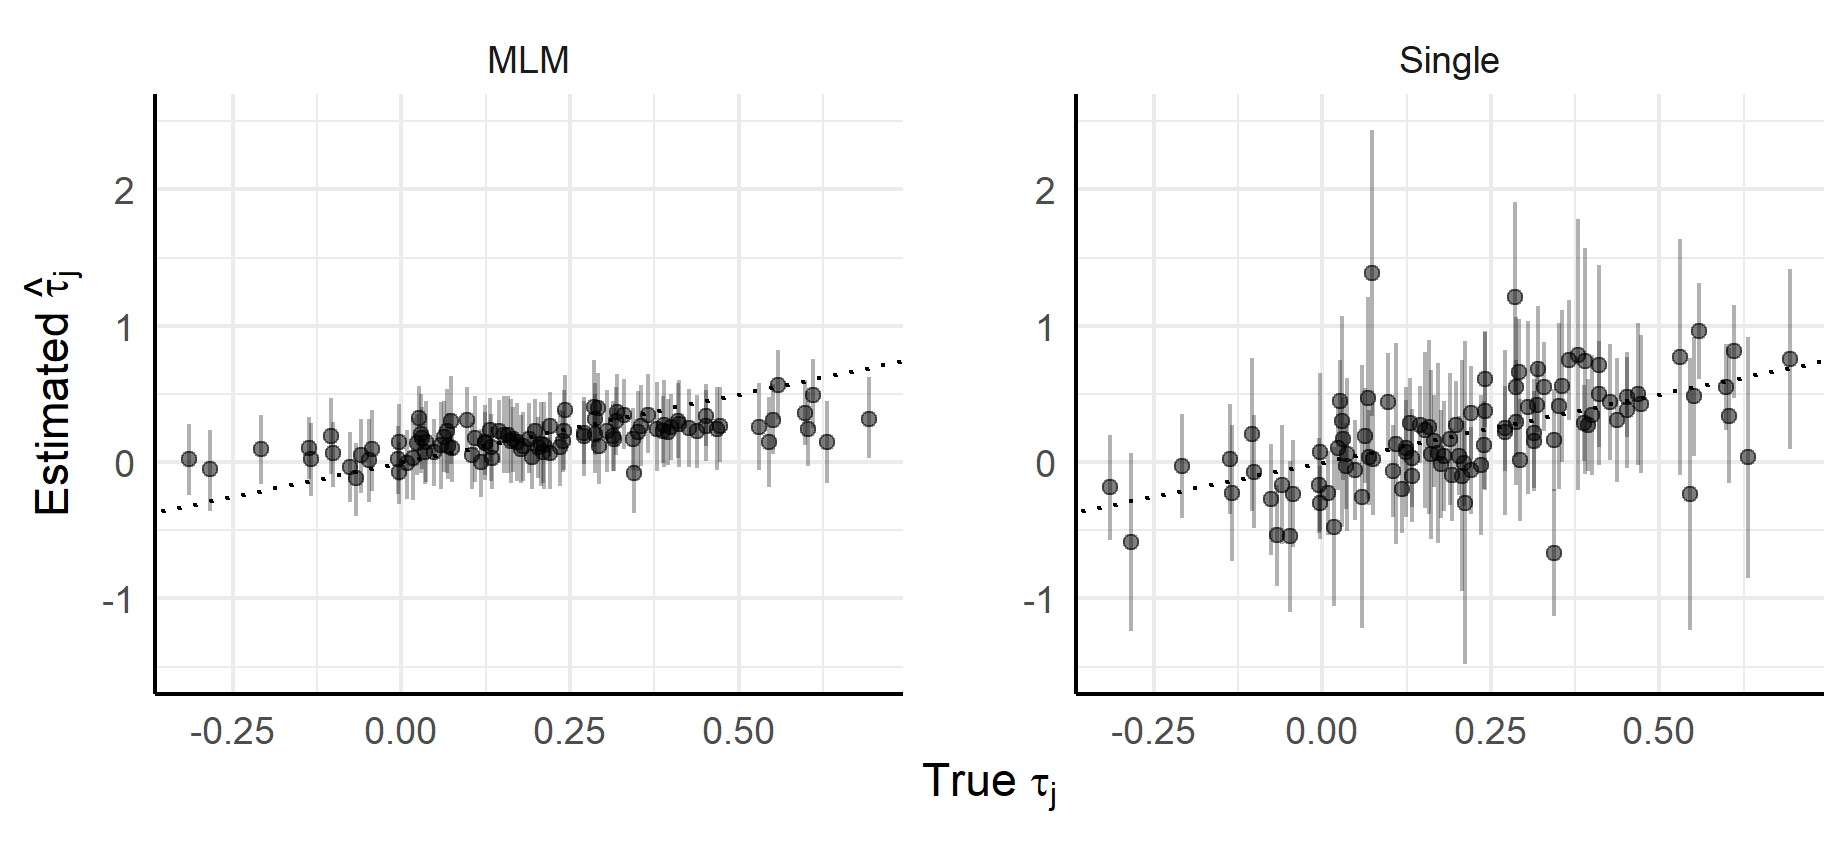
\includegraphics[width=\textwidth]{shrinkageplot}
	\caption{Interval estimates for one simulated dataset. Intervals overlapping the dotted line cover their respective true $\tau_j$ values.}
	\label{fig:shrinkageplot}
\end{figure}
In this simulation, 90 of the MLM intervals and 91 of the single-site intervals contain their respective true $\tau_j$ values.

The two methods, however, achieve this $\approx$ 90\% coverage in different ways.
As seen in Figure \ref{fig:shrinkageplot}, the MLM shrinks its point estimates toward the overall average.
This shrinkage improves coverage for moderate $\tau_j$ values, but causes the MLM to overestimate the lowest $\tau_j$ values and underestimate the highest $\tau_j$ values.
For example, Figure \ref{fig:shrinkageplot_slice1} highlights the intervals for sites with true $\tau_j \approx 0.6$.
\begin{figure}[ht]
	\centering
	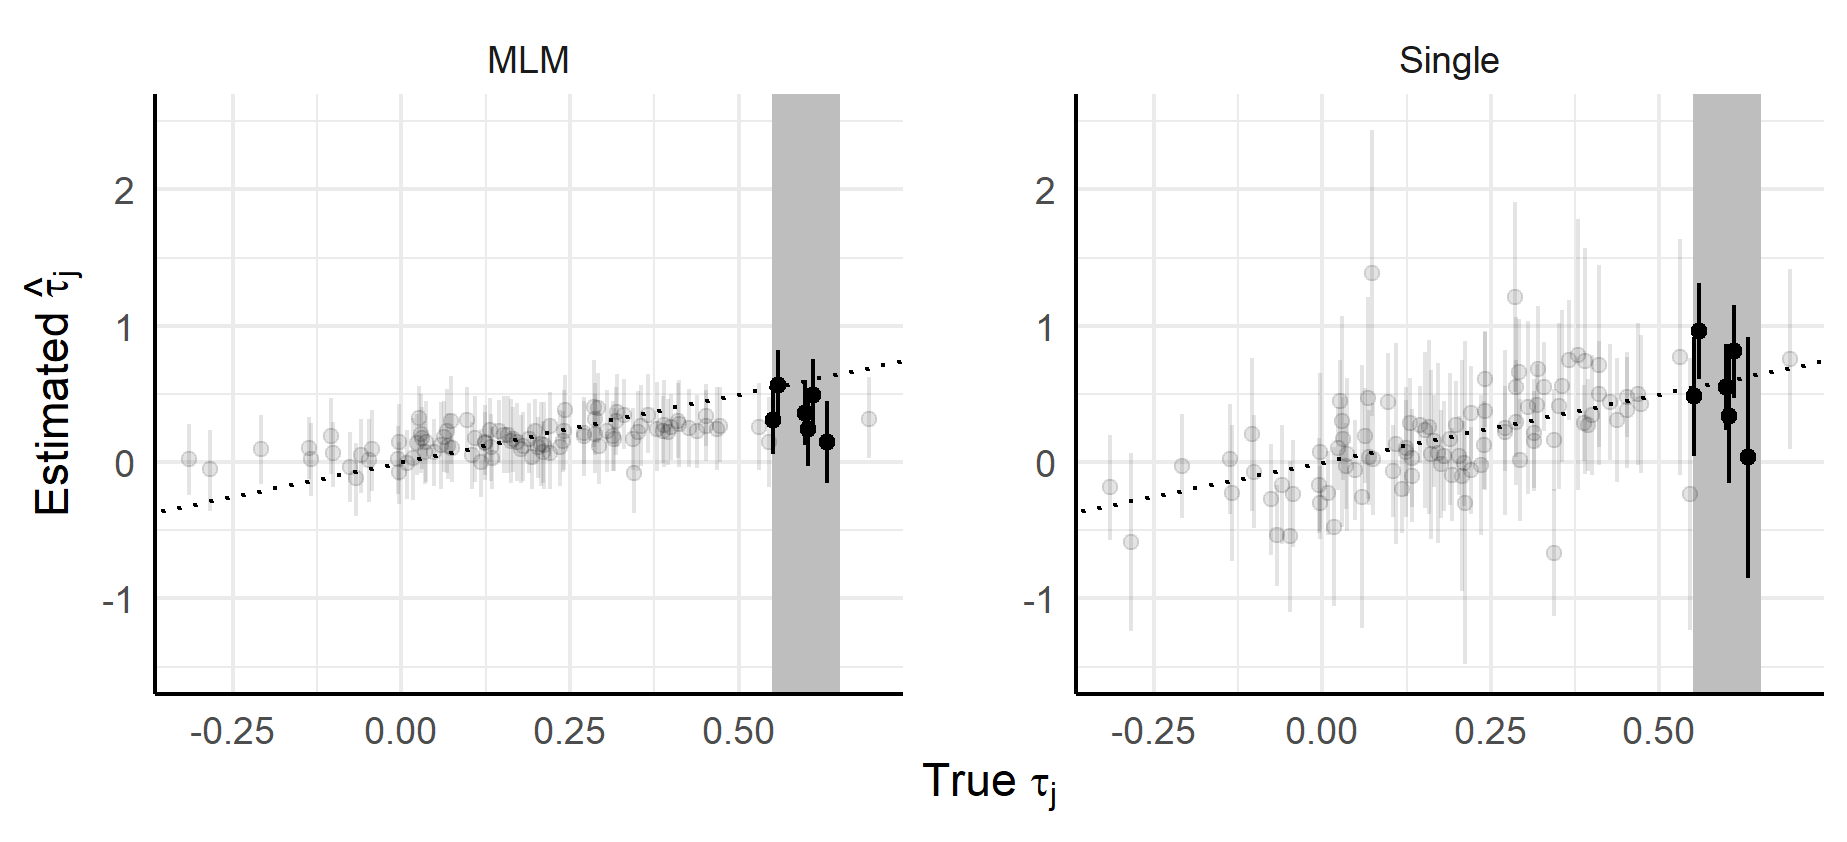
\includegraphics[width=\textwidth]{shrinkageplot_slice1}
	\caption{Interval estimates for one simulated dataset. Intervals for $\tau_j \approx 0.6$} are highlighted.
	\label{fig:shrinkageplot_slice1}
\end{figure}
While the single-site intervals are randomly scattered around the dotted line, shrinkage pulls the MLM intervals downward, causing many of them to fail to cover.

On the other hand, shrinkage ensures that when an MLM estimates that a site has a relatively extreme value of $\tau_j$, the site's true $\tau_j$ value is indeed likely to be extreme.
Figure \ref{fig:shrinkageplot_slice3} replicates Figure \ref{fig:shrinkageplot_slice1}, now highlighting intervals for sites with large estimated site-level treatment effects ($\hat{\tau}_j \approx 0.55$).
\begin{figure}[h]
	\centering
	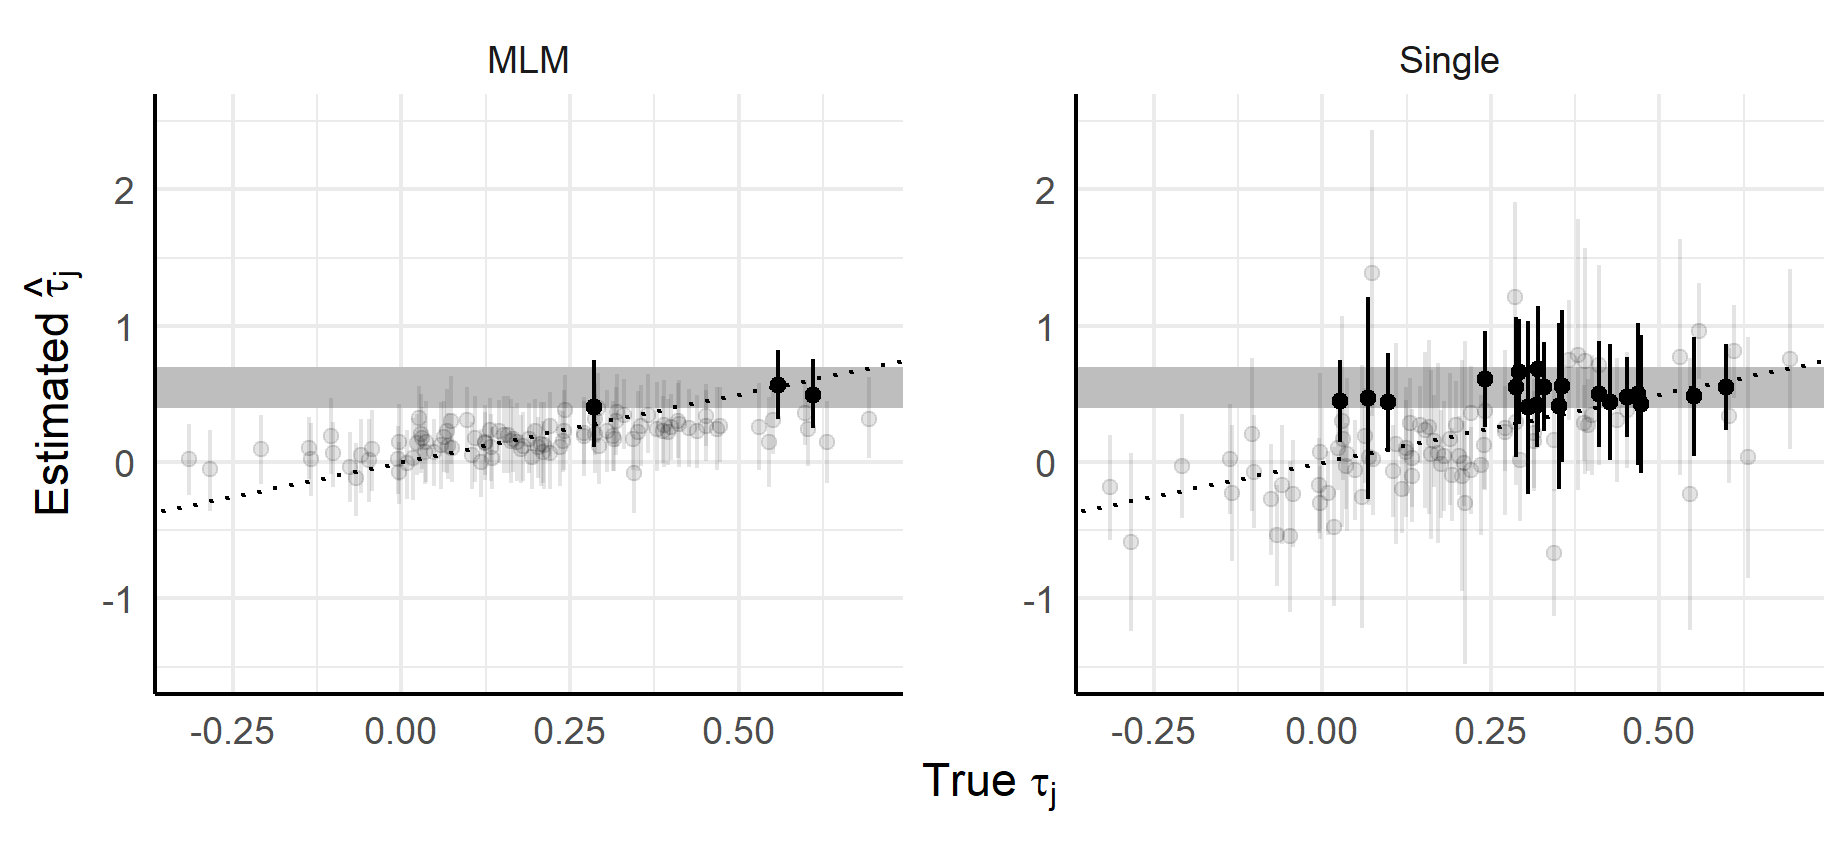
\includegraphics[width=\textwidth]{shrinkageplot_slice3}
	\caption{Interval estimates for one simulated dataset. Intervals for $\hat{\tau}_j \approx 0.55$ are highlighted.}
	\label{fig:shrinkageplot_slice3}
\end{figure}
We notice that the large MLM estimates are more clustered toward the right-hand side of the plot than are the large single-site estimates.
In other words, the large MLM estimates are more likely to correspond to truly large values of $\tau_j$.


\subsection{Repeated simulation}

To more precisely quantify these ideas of coverage for each $\tau_j$ value and coverage for each $\hat{\tau}_j$ value, we simulate 1000 multisite trial datasets and summarize the results in the figures below.
In a traditional power analysis, the analyst posits an effect size $c$ and computes power for that effect size.
An analogous procedure for the site-level treatment effects in a multisite trial is to compute power for each true site-level treatment effect size $\tau_j$.
Figure \ref{fig:pcp1} visualizes the results of a power simulation under this setup.\footnote{For clarity, we round the true site-level treatment effects $\tau_j$ to the nearest 0.05 prior to simulating site-level data, and we only visualize the power curves for $\tau_j =$ 0, 0.2, and 0.4.}
\begin{figure}[ht]
    \centering
    \begin{subfigure}[a]{\textwidth}
    	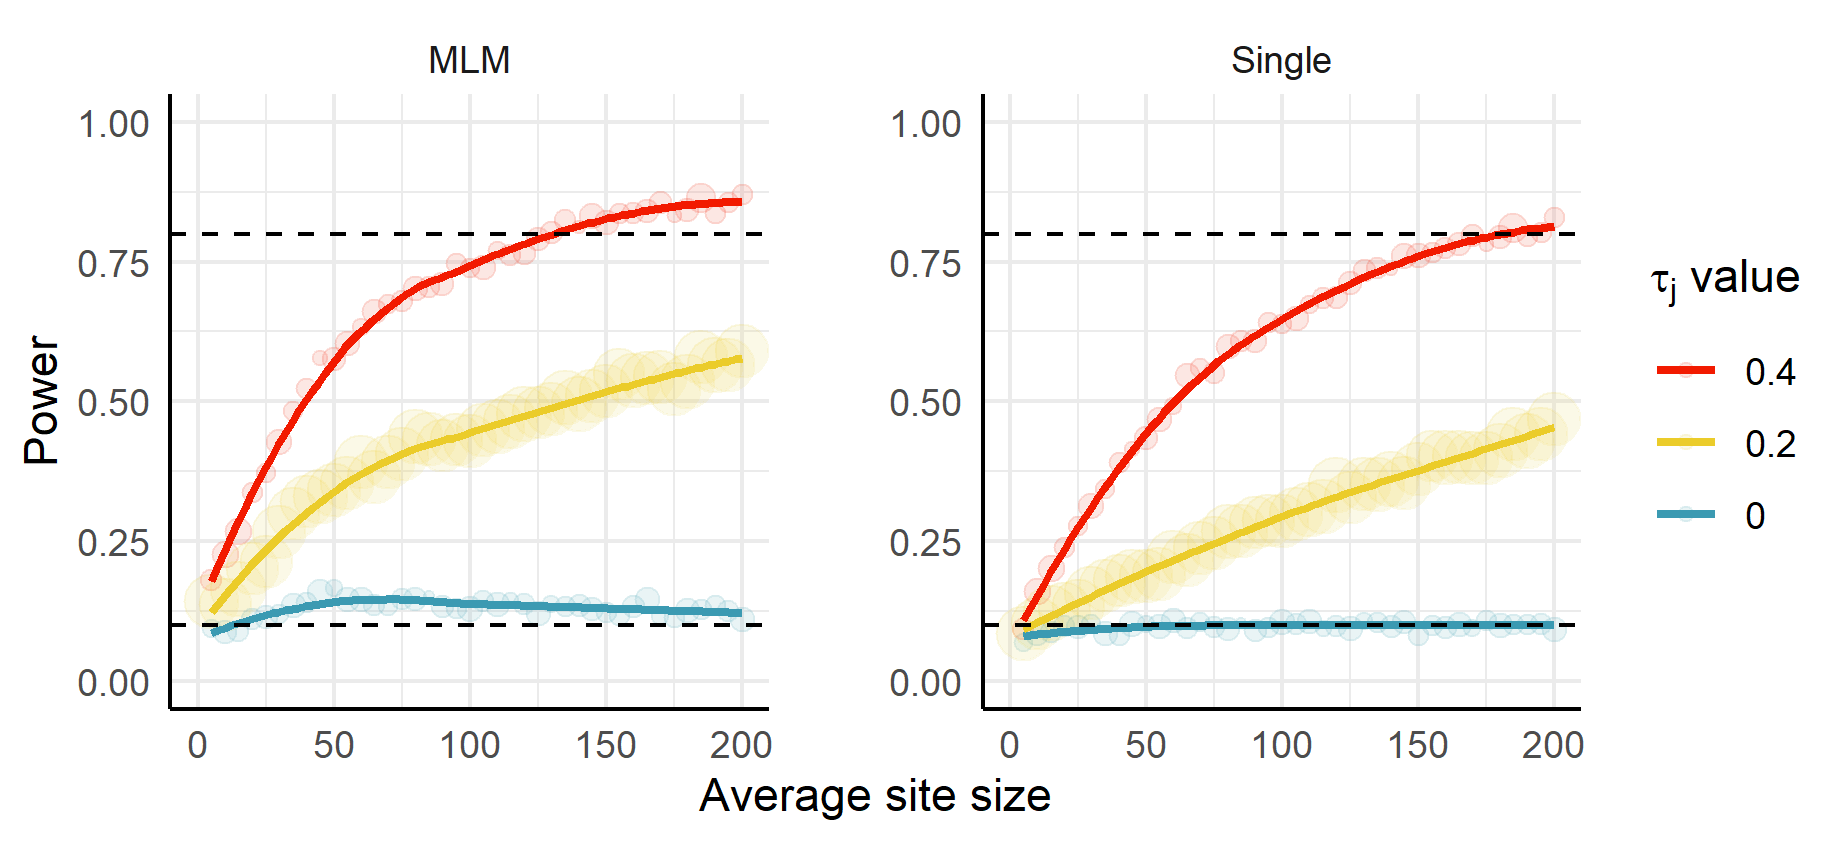
\includegraphics[width=\textwidth]{pp1}
        \caption{Rejection rate}
    	\label{fig:pp1}
    \end{subfigure}
    \vfill
    \begin{subfigure}[b]{\textwidth}
    	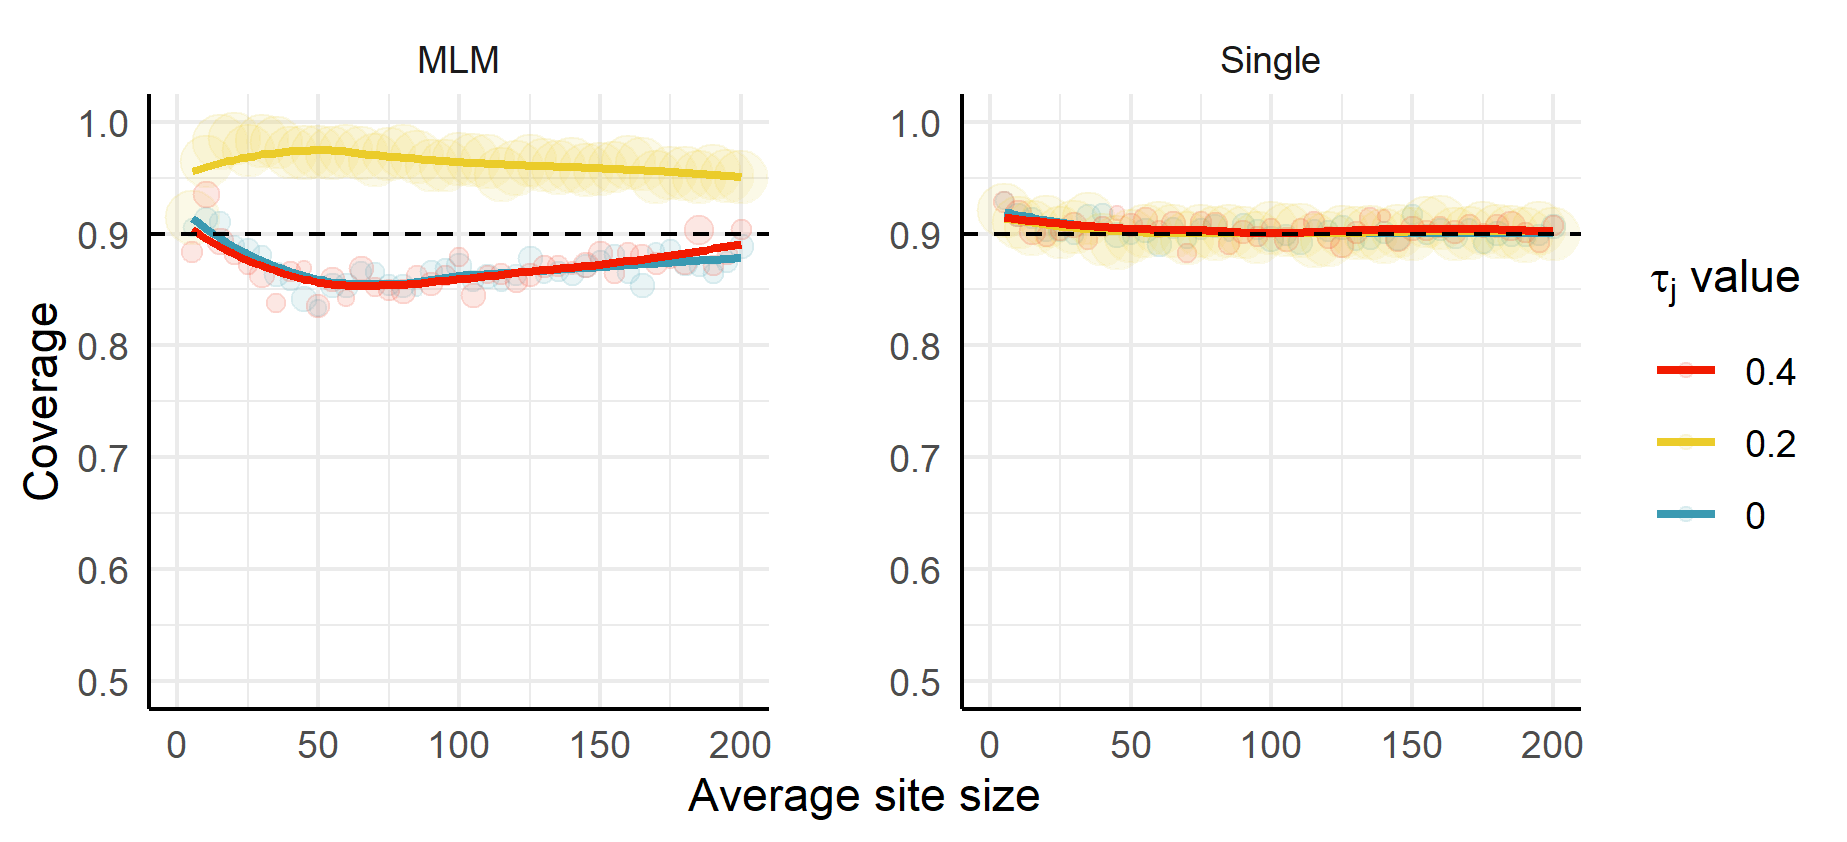
\includegraphics[width=\textwidth]{cp1}
        \caption{Coverage}
    	\label{fig:cp1}
    \end{subfigure}
    \caption{Power and coverage for $\tau_j = 0, 0.2, 0.4$ at $\alpha=0.1$, from 1000 simulations ($J=25$, ICC=0.2, $\tau=0.2$, $\sigma=0.2$).}
    \label{fig:pcp1}
\end{figure}
Figure \ref{fig:pp1} plots the average rejection rate against the average site size for sites with $\tau_j =$ 0, 0.2, and 0.4.
Clearly, MLMs improve power relative to the single-site interal estimates.
Unfortunately, we also notice that when $\tau_j = 0$, shrinkage causes MLMs to make false rejections at a rate higher than $\alpha=0.1$.
As previously noted, this is due to the fact that the interval estimates produced by MLMs undercover extreme values of $\tau_j$ (Figure \ref{fig:cp1}).

Figure \ref{fig:pp2} illustrates power conditional on \textit{estimated} site-level treatment effects $\hat{\tau}_j$.
\begin{figure}[ht]
    \centering
    \begin{subfigure}[a]{\textwidth}
    	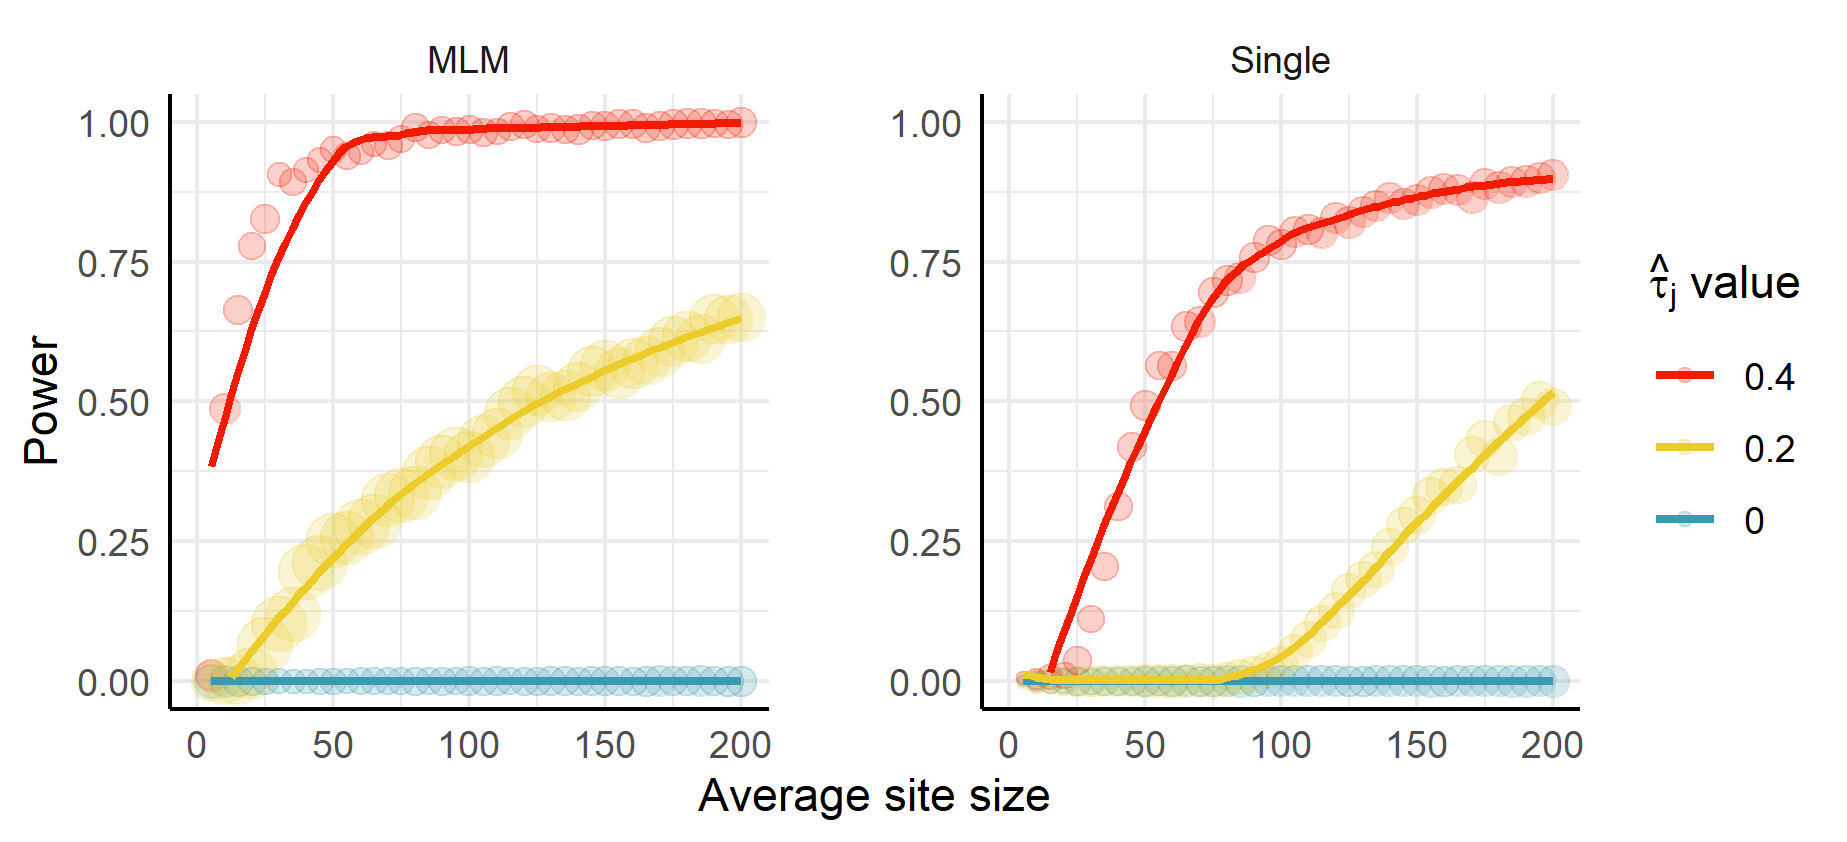
\includegraphics[width=\textwidth]{pp2}
        \caption{Rejection rate}
    	\label{fig:pp2}
    \end{subfigure}
    \vfill
    \begin{subfigure}[b]{\textwidth}
    	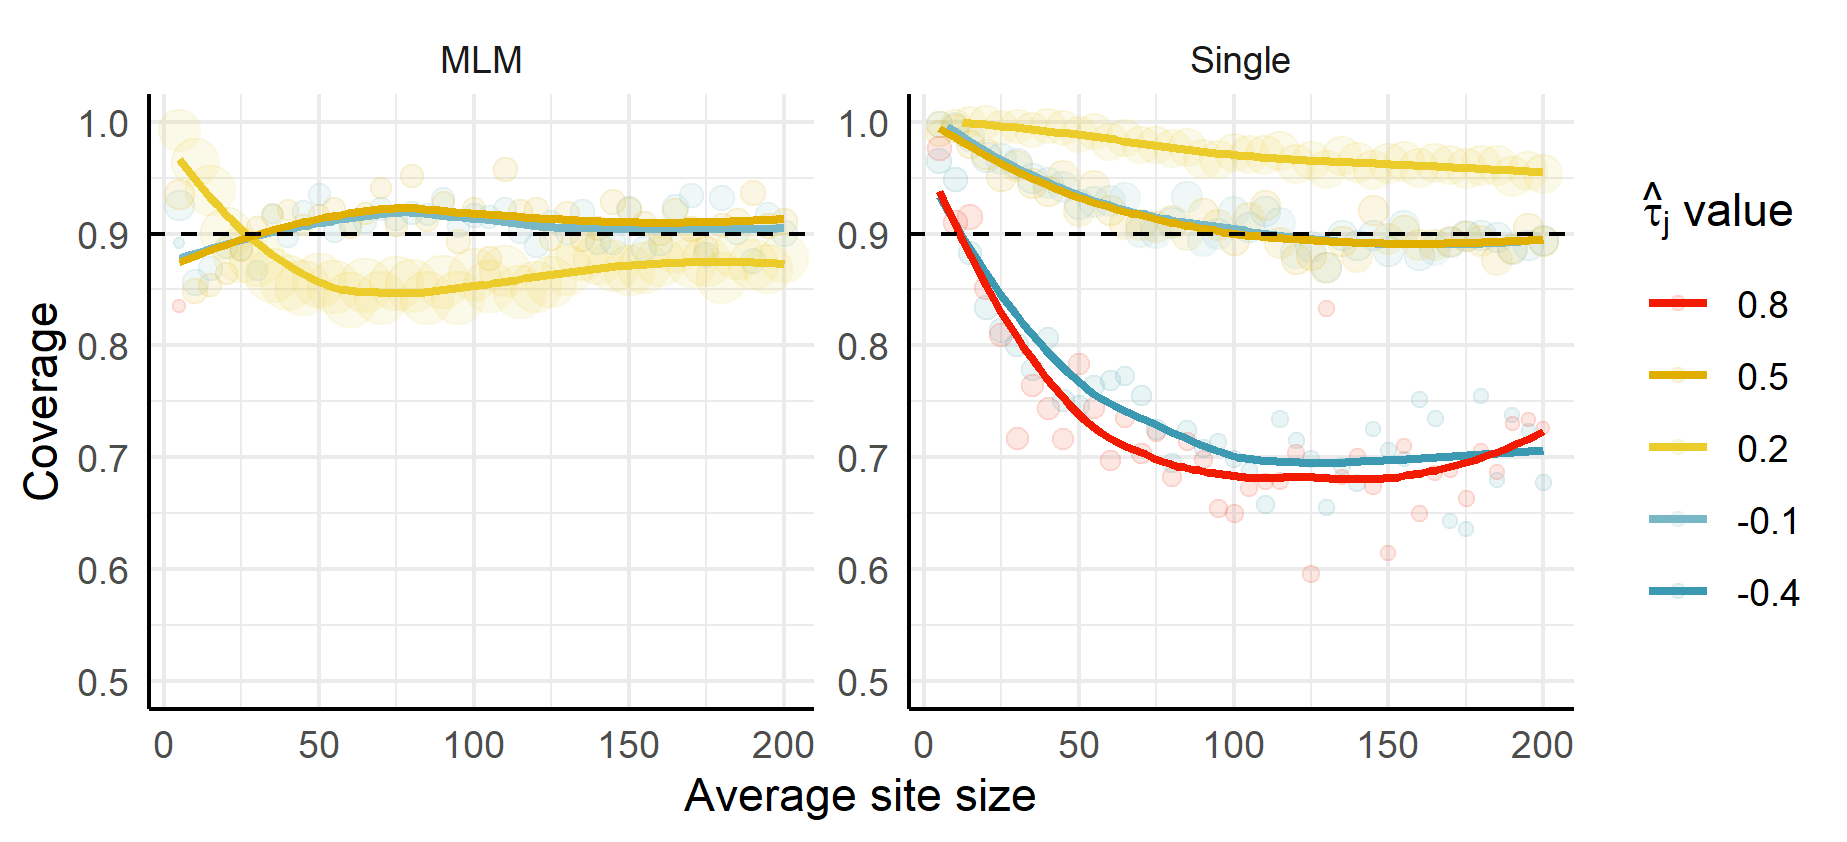
\includegraphics[width=\textwidth]{cp2}
        \caption{Coverage}
    	\label{fig:cp2}
    \end{subfigure}
    \caption{Power and coverage for $\hat{\tau}_j = 0, 0.2, 0.4$ at $\alpha=0.1$, from 1000 simulations ($J=25$, ICC=0.2, $\tau=0.2$, $\sigma=0.2$).}
    \label{fig:pcp2}
\end{figure}
We again notice that MLM intervals have better power than the single-site intervals.
Importantly, Figure \ref{fig:cp2}) shows that this increased power does not come at the cost of invalid tests; instead, we notice that while MLMs are approximately valid, the single-site intervals undercover, particularly for extreme estimated $\hat{\tau}_j$ values.
As shown in the illustrative example, the small sample sizes within each site cause single-site intervals to be noisy; as a result, they often estimate extreme $\hat{\tau}_j$ values for sites that do not have extreme true $\tau_j$ values, resulting in poor coverage across the collection of extreme interval estimates.
MLMs use shrinkage to avoid this problem.

\subsection{Initial conclusions}

Traditional power analyses help researchers compute the sample size needed to achieve 80\% power for a range of potential effect sizes.
As the example above demonstrates, however, this concept of ``potential effect sizes'' becomes unwieldy in multisite trials.
The empirical Bayes coverage targeted by many shrinkage methods targets average coverage across a distribution of effect sizes.
As a result, multilevel model intervals are invalid for particular true effect sizes $\tau_j$.
Without shrinkage, though, naive t-test intervals are too noisy to be reliable indicators of treatment effects.\footnote{Note that \cite{yu2018adaptive} provides intervals that are better... These work with very small sample sizes...? (interrogate Evan again)}

To avoid these challenges, we suggest that researchers focus on characterizing the average length of the interval estimates produced by their method of choice, across the posited distribution of $\tau_j$ values.
Averaging any metric of choice across the distribution of $\tau_j$ achieves two goals.
On a basic level, doing so mirrors the concept behind empirical Bayes coverage, which is what most shrinkage methods aim to achieve.
More practically, averaging across $\tau_j$ values circumvents the difficulties that come with conditioning on particular values of $\tau_j$, and may even be more useful for site-focused power analyses.
Prior to conducting a multisite trial, it is difficult to predict where a particular site's treatment effect $\tau_j$ may fall in the distribution $G$.
Since sites are exchangeable, however, analyzing the average performance of an interval estimator gives some indication of how that estimator will perform for each particular site, even without knowing $\tau_j$.

We suggest using interval length as the metric of choice to simplify interpretation.
We would ideally like to consider some form of average minimum detectable effect size (MDES), so that the multisite trial could be powered to consistently detect a particular effect size.
Unfortunately, it makes no sense to average MDES values across the distribution of $\tau_j$ values, since the MDES values themselves are the minimum $\tau_j$ values that achieve 80\% power.
Interval lengths, on the other hand, can be averaged across the distribution of $\tau_j$ values while still maintaining some of the primary motivations behind MDES.
Researchers can design a multisite trial to achieve some acceptable average margin of error for the site-level treatment effects.
Then, as a rule of thumb, the study would generally be powerful enough to detect effects larger than this average margin of error.
[NOTE: could do an interval length per $\tau_j$ value plot... essentially would show that $\tau_j=0.2$ has shorter intervals and extreme $\tau_j$ has wider intervals, not clear if this is helpful]

[One other motivation that I like, but it's not precise:
Average power begs the question: for which values of $\tau_j$ are the intervals more or less powerful?
This is a sad question, since conditioning on $\tau_j$ makes MLMs bad.
Average interval length, on the other hand, begs the question: for which values of $\hat{\tau}_j$ are the intervals longer or shorter?
This is a happier question.]


\section{Simulation study}

TONIGHT: run some simulations...

\subsection{Setup}

\subsection{Conclusions}


\section{Case study}

To illustrate our suggested approach for powering multisite trials to detect site-level treatment effects, we conduct an example power analysis.

[TODO: model this based on some application of interest, wait for ]


\section{Conclusion}

Synthesize simulation results here.

In many multisite trials, analysts may wish to power the trial to allow consistent detection of particular effect sizes at individual sites.
While this task appears straightforward prima facie, we need to be careful about...


\bibliography{refs.bib}
	
\end{document}